\documentclass{beamer}
\usepackage{amsmath,amsbsy,amsopn,amstext,amsfonts,amssymb}
\usepackage{isomath}
\usepackage{ulem}
%\linespread{1.6}  % double spaces lines
\usepackage{graphicx}
\usepackage{subfigure}
\usepackage{color}
\usepackage{optidef}  % define optimization problems
\usepackage{multicol}  % multiple columns
\usepackage{listings} % for python code
\usepackage{mathrsfs}

\usepackage{polynom}
\newcommand{\adj}{\mathrm{adj}}
\newcommand{\constrainedmin}[3]{
		\begin{mini*}|s|
		{#2}{#1}{}{}
		\addConstraint{#3}
		\end{mini*}
}

\newcommand{\rwbcomment}[1]{{\color{blue}RWB:#1}}
\newcommand{\defeq}{\stackrel{\triangle}{=}}
\newcommand{\abs}[1]{\left|#1\right|}
\newcommand{\norm}[1]{\left\|#1\right\|}
\newcommand{\iprod}[1]{\left<#1\right>}
\newcommand{\ellbf}{\boldsymbol{\ell}}
\newcommand{\nubf}{\boldsymbol{\nu}}
\newcommand{\mubf}{\boldsymbol{\mu}}
\newcommand{\abf}{\mathbf{a}}
\newcommand{\bbf}{\mathbf{b}}
\newcommand{\cbf}{\mathbf{c}}
\newcommand{\dbf}{\mathbf{d}}
\newcommand{\ebf}{\mathbf{e}}
\newcommand{\fbf}{\mathbf{f}}
\newcommand{\gbf}{\mathbf{g}}
\newcommand{\hbf}{\mathbf{h}}
\newcommand{\ibf}{\mathbf{i}}
\newcommand{\jbf}{\mathbf{j}}
\newcommand{\kbf}{\mathbf{k}}
\newcommand{\lbf}{\mathbf{l}}
\newcommand{\mbf}{\mathbf{m}}
\newcommand{\nbf}{\mathbf{n}}
\newcommand{\obf}{\mathbf{o}}
\newcommand{\pbf}{\mathbf{p}}
\newcommand{\qbf}{\mathbf{q}}
\newcommand{\rbf}{\mathbf{r}}
\newcommand{\sbf}{\mathbf{s}}
\newcommand{\tbf}{\mathbf{t}}
\newcommand{\ubf}{\mathbf{u}}
\newcommand{\vbf}{\mathbf{v}}
\newcommand{\wbf}{\mathbf{w}}
\newcommand{\xbf}{\mathbf{x}}
\newcommand{\ybf}{\mathbf{y}}
\newcommand{\zbf}{\mathbf{z}}
\newcommand{\Jbf}{\mathbf{J}}
\newcommand{\Acal}{\mathcal{A}}
\newcommand{\Bcal}{\mathcal{B}}
\newcommand{\Lcal}{\mathcal{L}}
\newcommand{\Ncal}{\mathcal{N}}
\newcommand{\Rcal}{\mathcal{R}}
\definecolor{darkolivegreen}{rgb}{0.33, 0.42, 0.18}

\makeatletter
\newenvironment<>{proofstart}[1][\proofname]{%
    \par
    \def\insertproofname{#1\@addpunct{.}}%
    \usebeamertemplate{proof begin}#2}
  {\usebeamertemplate{proof end}}
\newenvironment<>{proofcont}{%
  \setbeamertemplate{proof begin}{\begin{block}{}}
    \par
    \usebeamertemplate{proof begin}}
  {\usebeamertemplate{proof end}}
\newenvironment<>{proofend}{%
    \par
    \pushQED{\qed}
    \setbeamertemplate{proof begin}{\begin{block}{}}
    \usebeamertemplate{proof begin}}
  {\popQED\usebeamertemplate{proof end}}
\makeatother

\title{ECEn 671: Mathematics of Signals and Systems}
\author{Randal W. Beard}
\institute{Brigham Young University}
\date{\today}

\begin{document}

%-------------------------------
\begin{frame}
	\titlepage
\end{frame}



%%%%%%%%%%%%%%%%%%%%%%%%%%%%%%%%%%%%%%%%%%%%%%%%%%%%%%%%%%%%%%%%%
\section{Eigenfilters}
\frame{\sectionpage}

%----------------------------------
\begin{frame}\frametitle{Eigenfilters for Random Signals}
	{\color{blue}Problem:}
	Given
	\begin{center}
		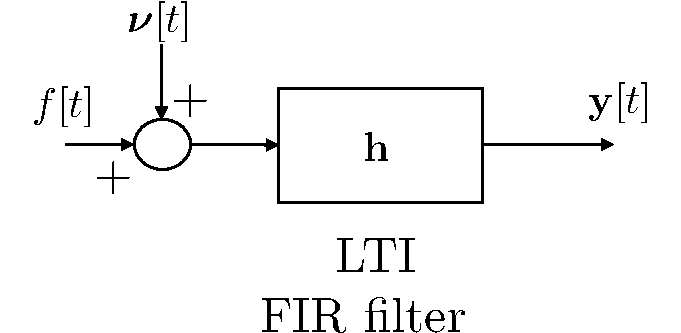
\includegraphics[width=0.6\textwidth]{figures/chap6_eigenfilter}
	\end{center}
	where $\nu$ is white noise with variance $\sigma^2$, and $f$ is a stationary, zero-mean random process.
	
	\vfill
	
	Find $\mathbf{h}$ to maximize the signal-to-noise ratio.
\end{frame}

%----------------------------------
\begin{frame}\frametitle{Eigenfilters for Random Signals}
	Let
	\[
		\fbf(t) 
			= \begin{pmatrix}
	    		f(t)\\
	    		f(t-1)\\
	    		\vdots\\
	    		f(t-(m-1))
	  		  \end{pmatrix}
	\]
	then
	\[ 
		y(t) = \hbf^H \fbf(t).
	\]
	The output power due to the signal $\fbf$ is 
	\begin{align*}
		P_0 
		&= E|y(t)|^2 = E|\hbf^H\fbf(t)|^2 = E\{\hbf^H\fbf(t)\hbf^H\fbf(t)\}\\
		&= E\{\hbf^H\fbf(t)\fbf^H(t)\hbf\}= \hbf^HE\{\fbf(t)\fbf^H(t)\}\hbf\\
		&= \hbf^HR\hbf
	\end{align*}
	
	where $R = E\{\fbf(t) \fbf^H(t)\} $
\end{frame}

%----------------------------------
\begin{frame}\frametitle{Eigenfilters for Random Signals}
	Let 
	\[ 
		\nubf(t) 
			= \begin{pmatrix}
	    		v(t)\\
	    		v(t-1)\\
	    		\vdots
	    		\\
	    		v(t-m+1)
	  		  \end{pmatrix}
	\]
	Then the output due to the noise is
	\[ 
		\hbf\nubf(t) 
	\]
	and the average noise power is
	\[ 
		N_0 = E\{\hbf^H\nubf(t)\nubf^H(t)\hbf\} 
		    = \sigma^2\hbf^H\hbf 
	\]
\end{frame}

%----------------------------------
\begin{frame}\frametitle{Eigenfilters for Random Signals}
	The signal-to-noise ratio is
	\begin{align*}
		SNR &= \frac{P_0}{N_0} \\
		    &= \frac{1}{\sigma^2} \cdot
		    	\underbrace{
		    		\frac{\hbf^HR\hbf}{\sigma^2\hbf^H\hbf}
		    	}_{\text{Rayleigh quotient}} 
	\end{align*}
	Therefore
	\[ 
		SNR_{max} = \frac{\lambda_1}{\sigma^2} 
	\]
	where $\lambda_1$ is the largest eigenvalue of $R$ and $\hbf = q_1$ the largest eigenvector of $R$.
\end{frame}


\end{document}